% !TeX root = ../../Book5.tex
% * 状态：初稿已完成；正文、证明、算例与配套习题解答已写齐，尚未正式审核。
% 纲要标题：### F.3 旗与楼的模型
% 写作状态：初稿已完成；新增内容尚未正式审核。
% 写作范围：A 型旗复形及其公寓公理、低秩模型与余维一邻接；不展开一般楼理论。
% #### F.3.1 旗与旗复形
% #### F.3.2 楼的低秩模型
% #### F.3.3 公寓、室与余维一邻接

\section{旗与楼的模型}
\label{b5:sec:F03}

Bruhat 分解用一个置换记录两面完全旗的相对位置。若还想看见只改变旗中一个子空间时发生了什么，就应把完全旗和它们共有的部分旗一起保留。由子空间的包含关系构成的复形正好记录这些资料。选定一组基后，坐标子空间给出其中一个有限模型；让基变化，这些模型便覆盖整个旗复形。这是一般线性群的楼可以直接从线性代数中构造出来的原因。

\subsection{旗与旗复形}
\label{b5:subsec:F03:01}

在三维空间中，一维子空间可以包含于许多二维子空间。若把每个非零真子空间看成一个顶点，并在有包含关系的两个顶点之间连边，一面完全旗便成为一条边。四维时，完全旗有三个非零真子空间，应记录为一个包含内部的三角形，而不只是它的三条边；更高维的旗则需要相应的高维单纯形。

\begin{definition}\label{b5:def:F-flag-complex}
	设 \(\mathcal V\) 为集合，\(\Delta\) 为由 \(\mathcal V\) 的有限子集组成的非空集合族。若每个单点集属于 \(\Delta\)，且 \(\sigma\in\Delta\)、\(\tau\subseteq\sigma\) 蕴涵 \(\tau\in\Delta\)，则 \(\Delta\) 称为\term[chouxiang-danchun-fuxing]{抽象单纯复形}[abstract simplicial complex]。\(\mathcal V\) 中的元素称为顶点，\(\Delta\) 中的元素称为单纯形；\(\sigma\) 的维数为 \(\lvert\sigma\rvert-1\)，包含于它的单纯形称为它的面。特别地，空集是维数 \(-1\) 的面。

	设 \(V\) 为域 \(k\) 上的 \(n\) 维向量空间，\(n\ge2\)。以非零真子空间 \(0<U<V\) 为顶点，以有限的严格包含链为单纯形，所得复形记为 \(\Delta(V)\)，称为 \(V\) 的\term[qi-fuxing]{旗复形}[flag complex]。顶点 \(U\) 的型为 \(\dim_kU\)，一面旗的型是其中各子空间维数所成的集合。
\end{definition}
\symidx{\(\Delta(V)\)：向量空间的旗复形}

这里链可看成子空间的集合，因为包含关系已经唯一确定了它们的排列顺序。删除链中的任意若干项仍是一条链，因此它们确实组成单纯复形。文献也把偏序集所有有限链组成的复形称为该偏序集的序复形；这里采用子空间偏序集的这一构造。

\begin{proposition}\label{b5:prop:F-chambers-flags}
	设 \(V\) 为域 \(k\) 上的 \(n\) 维向量空间，\(n\ge2\)。\(\Delta(V)\) 的极大单纯形恰为完全旗
	\[
		0=V_0<V_1<\cdots<V_{n-1}<V_n=V,
		\qquad \dim_kV_i=i,
	\]
	其中 \(0,V\) 仅用于补全记号，不算复形的顶点。每个单纯形都包含于一个这样的极大单纯形，故 \(\Delta(V)\) 的所有极大单纯形均有维数 \(n-2\)。
\end{proposition}

\begin{proof}
	若链中相邻两项 \(U<W\) 的维数之差大于 \(1\)，则取 \(w\in W\setminus U\)，有 \(U<U+kw<W\)，可以继续插入子空间。对链两端也把 \(0,V\) 暂时加入并作同样处理。维数严格递增且介于 \(0,n\) 之间，这个过程有限步结束，得到各维数均出现的完全旗。反之，一条完全旗已经包含每一种非零真子空间维数，不可能再插入子空间。因此它恰为极大单纯形，有 \(n-1\) 个顶点，维数为 \(n-2\)。
\end{proof}

\begin{definition}\label{b5:def:F-chamber-panel}
	设 \(\Delta\) 为单纯复形，所有极大单纯形均有 \(r\ge1\) 个顶点。它的极大单纯形称为\term[shi-lou]{室}[chamber]。从一室中删去恰好一个顶点所得的面称为\term[yu-wei-yi-mian]{余维一面}[panel]。

	在域 \(k\) 上的 \(n\) 维向量空间 \(V\) 的旗复形中，\(n\ge2\)，有 \(r=n-1\)。若删去的是 \(i\) 维子空间，就称所得余维一面缺少型 \(i\)。两个不同的室若恰好在 \(i\) 维子空间处不同，则称它们为 \(i\)-相邻；不指定 \(i\) 时简称相邻。
\end{definition}

室有 \(n-1\) 个顶点，余维一面有 \(n-2\) 个顶点。当 \(n=2\) 时，室本身就是顶点，余维一面是空面，因此任意两个不同的室都相邻。这一约定使秩一的情形也能使用同一组定义。

\ProseParagraphBreak

\(\operatorname{GL}(V)\) 对子空间的作用保持维数和包含关系，因而作用于 \(\Delta(V)\)。一室的稳定子就是相应的旗稳定子；选取适配基后，它成为可逆上三角矩阵群 \(B\)。前一节的 \(G/B\) 因此是室的集合，而部分旗对应的陪集空间还记住了室的各类面。复形把这些集合之间的遗忘映射合在了同一个包含结构中。

\subsection{楼的低秩模型}
\label{b5:subsec:F03:02}

取 \(V\) 的一组基 \(\mathcal E=(e_1,\ldots,e_n)\)。对每个非空真子集 \(I\subset\{1,\ldots,n\}\)，令
\[
	V_I=\operatorname{span}_k\{\,e_i\mid i\in I\,\}.
\]
以这些坐标子空间为顶点，以它们的包含链为单纯形，得到 \(\Delta(V)\) 的子复形 \(\mathcal A_{\mathcal E}\)。它只依赖无序的一维子空间组 \(\{ke_1,\ldots,ke_n\}\)，而不依赖各 \(e_i\) 的非零倍数。这样的子复形称为\term[gongyu]{公寓}[apartment]。
\symidx{\(\mathcal A_{\mathcal E}\)：由一组基给出的坐标公寓}

\ProseParagraphBreak

由于 \(V_I\subseteq V_J\) 当且仅当 \(I\subseteq J\)，每个坐标公寓都同构于 \(\{1,\ldots,n\}\) 的非空真子集所成的链复形，模型中子集 \(I\) 的型为 \(\lvert I\rvert\)。这个有限复形是 \(A_{n-1}\) 型的\term[Coxeter-fuxing]{Coxeter 复形}[Coxeter complex]：它的一室由一个排列 \(w\in S_n\) 给出，链中的指标集依次为
\[
	\{w(1)\}\subset\{w(1),w(2)\}\subset\cdots
	\subset\{w(1),\ldots,w(n-1)\}.
\]
反过来，逐次找出链中新增加的指标便恢复 \(w\)，所以每个公寓恰有 \(n!\) 个室。这个模型也可以看成一个 \((n-1)\) 维单纯形边界的重心细分，因而其几何实现是 \((n-2)\) 维球面；“球面型”所指的是公寓模型，而不是说整个楼是一张球面。

\ProseParagraphBreak

当 \(n=2\) 时，\(\Delta(V)\) 的顶点是一维子空间，即射影直线 \(\mathbb P^1(k)\) 的点。任意两个不同的一维子空间之和等于 \(V\)，所以它们构成一个公寓。公寓只有两个点，这是零维球面；整个复形则没有边。若 \(k=\mathbb F_q\)，其室数为
\[
	\lvert\mathbb P^1(\mathbb F_q)\rvert
	=\frac{q^2-1}{q-1}=q+1.
\]
分子数的是非零向量，分母是每个一维子空间中的非零向量数。

\ProseParagraphBreak

当 \(n=3\) 时，把一维子空间称为射影点，把二维子空间称为射影直线。旗复形是一张二部图：顶点分成点和直线两类，边表示一个点落在一条直线上。选定基后，记 \(P_i=ke_i\)、\(H_{ij}=ke_i+ke_j\)。对应公寓是六边形
\[
	P_1-H_{12}-P_2-H_{23}-P_3-H_{13}-P_1.
\]
每条边是一室，每个顶点是余维一面；六边形围成的区域不属于这个一维复形。\cref{b5:fig:F-A2-apartment}还画出了一个公寓之外的邻接：\(H'=ke_1+k(e_2+e_3)\) 包含 \(P_1\)，但不是坐标子空间。

\begin{figure}[htbp]
	\centering
	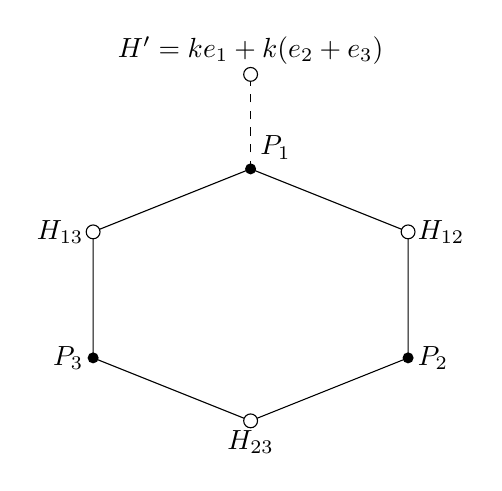
\begin{tikzpicture}
		\coordinate (P1) at (0,1.6);
		\coordinate (H12) at (2,0.8);
		\coordinate (P2) at (2,-0.8);
		\coordinate (H23) at (0,-1.6);
		\coordinate (P3) at (-2,-0.8);
		\coordinate (H13) at (-2,0.8);
		\coordinate (Hp) at (0,2.8);
		\draw (P1)--(H12)--(P2)--(H23)--(P3)--(H13)--cycle;
		\draw[dashed] (P1)--(Hp);
		\foreach \p in {P1,P2,P3} {\fill (\p) circle (2pt);}
		\foreach \h in {H12,H23,H13,Hp} {\draw[fill=white] (\h) circle (2.5pt);}
		\node[above right] at (P1) {\(P_1\)};
		\node[right] at (H12) {\(H_{12}\)};
		\node[right] at (P2) {\(P_2\)};
		\node[below] at (H23) {\(H_{23}\)};
		\node[left] at (P3) {\(P_3\)};
		\node[left] at (H13) {\(H_{13}\)};
		\node[above] at (Hp) {\(H'=ke_1+k(e_2+e_3)\)};
	\end{tikzpicture}
	\caption[\(A_2\) 型坐标公寓]{\(A_2\) 型坐标公寓。实心点表示一维子空间，空心点表示二维子空间；实线六边形是一个公寓，虚线是一条离开该公寓的旗。}
	\label{b5:fig:F-A2-apartment}
\end{figure}

这些公寓彼此重叠。要使它们能够一致地描述不同位置的旗，除了每个公寓具有相同模型以外，还需要两条相容条件。

\begin{definition}\label{b5:def:F-A-building}
	设 \(n\ge2\)，\(\Delta\) 为一个单纯复形，其顶点带有 \(1,\ldots,n-1\) 中的型，每个单纯形的顶点型互不相同。给定一族子复形 \(\mathscr A\)，其中每个成员都保型同构于 \(A_{n-1}\) 型的上述子集链复形。若满足以下条件，则称 \((\Delta,\mathscr A)\) 为一个 \(A_{n-1}\) 型的\term[lou]{球面楼}[spherical building]，其秩为 \(n-1\)：
	\begin{enumerate}
		\item 任意两个单纯形都包含于某个公寓中。
		\item 对任意两个公寓 \(\mathcal A,\mathcal A'\)，存在保型的复形同构 \(\mathcal A\to\mathcal A'\)，使两者交集中每个顶点保持不变。
	\end{enumerate}
	这里复形同构是顶点集合的双射，要求它和它的逆都把单纯形送到单纯形；保型是指不改变顶点的型。
\end{definition}

定义中的秩是室的顶点数；相应复形的维数比秩少 \(1\)。本节只使用这一 \(A\) 型模型。一般球面楼以其他有限 Coxeter 群的复形取代子集链复形；其公寓公理及与 BN 对的关系可参看\cite[Chapter 9, pp. 97--100]{Taylor1992ClassicalGroups}。

\begin{theorem}\label{b5:thm:F-vector-building}
	设 \(V\) 为域 \(k\) 上的 \(n\) 维向量空间，\(n\ge2\)。旗复形 \(\Delta(V)\) 连同所有坐标公寓构成一个 \(A_{n-1}\) 型球面楼。
\end{theorem}

\begin{proof}
	每个坐标公寓已经由 \(I\mapsto V_I\) 与子集链模型保型同构。给定两个单纯形，由\cref{b5:prop:F-chambers-flags}把它们分别补成完全旗。\cref{b5:lem:F-common-flag-basis}给出同时适配这两面完全旗的一组基，因此两面旗和原来的两个单纯形均包含于该基的坐标公寓。这证明第一条公理。

	第二条公理要求同时固定所有共有子空间，而不只是选择一面共有旗。设两个公寓分别由基 \((e_1,\ldots,e_n)\)、\((f_1,\ldots,f_n)\) 给出，写
	\[
		f_j=\sum_{i=1}^n a_{ij}e_i,
		\qquad A=(a_{ij})\in\operatorname{GL}_n(k).
	\]
	由于 \(\det A\ne0\)，其行列式展开中至少有一项非零，所以可以选择 \(\sigma\in S_n\)，使 \(a_{\sigma(j),j}\ne0\) 对每个 \(j\) 都成立。由 \(f_j\mapsto e_{\sigma(j)}\) 定义线性同构 \(T:V\to V\)。它把 \(f\) 基的坐标子空间送到 \(e\) 基的坐标子空间，因而给出公寓之间的保型复形同构。

	设 \(U\) 是这两个公寓共有的顶点。存在唯一指标集 \(I,J\)，使
	\[
		U=\operatorname{span}_k\{\,e_i\mid i\in I\,\}
		 =\operatorname{span}_k\{\,f_j\mid j\in J\,\}.
	\]
	若 \(j\in J\)，则 \(f_j\in U\)，故 \(a_{ij}=0\) 对每个 \(i\notin I\) 成立。选出的非零项迫使 \(\sigma(j)\in I\)，于是 \(\sigma(J)\subseteq I\)。又 \(\lvert I\rvert=\dim U=\lvert J\rvert\)，从而 \(\sigma(J)=I\)，即 \(T(U)=U\)。同一个 \(T\) 对每个共有顶点都满足这一等式，因此它在公寓交集上固定全部顶点。取其逆即得定义所需方向的同构。这里固定的是作为顶点的子空间，不要求 \(T\) 固定该子空间中的每个向量。
\end{proof}

上述证明把“两旗有共同适配基”与“两个坐标模型能在交集上相合”分开处理。前者控制两室的相对位置，后者保证换公寓时共同的面仍表示同一个子空间。有限域只在计数时才是必要条件，楼的这项线性代数构造对任意域都成立。

\subsection{公寓、室与余维一邻接}
\label{b5:subsec:F03:03}

在一个坐标公寓中，固定除 \(i\) 维子空间以外的全部旗项，补回这一项只有两种坐标选择；在整个旗复形中却有更多选择。这个差别可以在一个二维商空间内完全算清。

\begin{proposition}\label{b5:prop:F-panel-count}
	设 \(V\) 为 \(\mathbb F_q\) 上的 \(n\) 维向量空间，\(n\ge2\)。\(\Delta(V)\) 的每个余维一面恰包含于 \(q+1\) 个室中；若该面位于一个固定公寓，则其中恰有两个室属于该公寓。因此，每个室对每种型 \(i\in\{1,\ldots,n-1\}\) 恰有 \(q\) 个不同的 \(i\)-相邻室，总共有 \((n-1)q\) 个相邻室。
\end{proposition}

\begin{proof}
	设给定的余维一面缺少型 \(i\)。把端点补成 \(V_0=0,V_n=V\)，其两侧已给定的子空间是 \(V_{i-1}<V_{i+1}\)。补回一室等价于选择
	\[
		V_{i-1}<W<V_{i+1},\qquad \dim W=i.
	\]
	映射 \(W\mapsto W/V_{i-1}\) 将这些选择与二维空间 \(V_{i+1}/V_{i-1}\) 中的一维子空间一一对应，逆映射是取商映射下的原像。后一集合有 \((q^2-1)/(q-1)=q+1\) 个元素。

	若余维一面位于一个固定坐标公寓，则代表 \(V_{i+1}\) 的坐标指标集比代表 \(V_{i-1}\) 的指标集恰多两个指标。在公寓内补回 \(W\)，只能先加入其中一个指标，故恰有两个选择。固定一个室后，其中一个选择是原室；在整个楼内，其余 \(q\) 个选择才是不同的相邻室。不同型的相邻室改变的是不同维数的旗项，不会重复计算，所以总数为 \((n-1)q\)。
\end{proof}

每个余维一面恰含于两个室的复形称为\term[bao-fuxing]{薄复形}[thin complex]；若每个余维一面至少含于三个室，则称为\term[hou-fuxing]{厚复形}[thick complex]。所以公寓是薄的，而 \(\Delta(\mathbb F_q^n)\) 是厚的。\cref{b5:fig:F-A2-apartment}中 \(P_1\) 在公寓内只连着 \(H_{12},H_{13}\)，但整个楼至少还有 \(H'\) 这一选择。当 \(q=2\) 时，三个选择恰好全部画出。

\ProseParagraphBreak

公寓的室用排列 \(w\) 编号时，\(i\)-相邻恰好交换排列列表中第 \(i\)、\(i+1\) 两项，即把 \(w\) 换成 \(ws_i\)，其中 \(s_i=(i\ i+1)\)。这是因为只交换这两个指标，会且只会改变由前 \(i\) 个基向量张成的子空间。任意排列都可由相邻换位得到，所以公寓内任意两室可以经有限次余维一邻接相连。任意两室又同处某个公寓，故整个旗复形的室也具有这一连通性。\(A_2\) 公寓的六个室依次围成一圈，从一室到对面一室的两条三步路径分别具有型序列 \((1,2,1)\) 与 \((2,1,2)\)，对应于 \(s_1s_2s_1=s_2s_1s_2\)。

\ProseParagraphBreak

这里有两张应当区别的图。三维时，旗复形本身的顶点是射影点和射影直线，室是它的边；若另外把室作为顶点、把余维一邻接作为边，就得到室的邻接图。固定一个余维一面的 \(q+1\) 个室在后一张图中两两相邻，所以会出现三角形；这不表示原来的点线关联图中也出现了三角形。后一种邻接将用于下一节定义旗上的算子，而其中的参数 \(q\) 正是每个给定型的不同相邻室数。
